\graphicspath{{./figures}}

\section{High-Level System}
There are various decisions to be made regarding the entire communication system. A complete high-level system block diagram illustrating the decisions discussed below is shown in Figure \ref{fig:complete_system}. Note that the yellow blocks are external (i.e. assumed to be available already).

\begin{figure}[!htb]
    \centering
    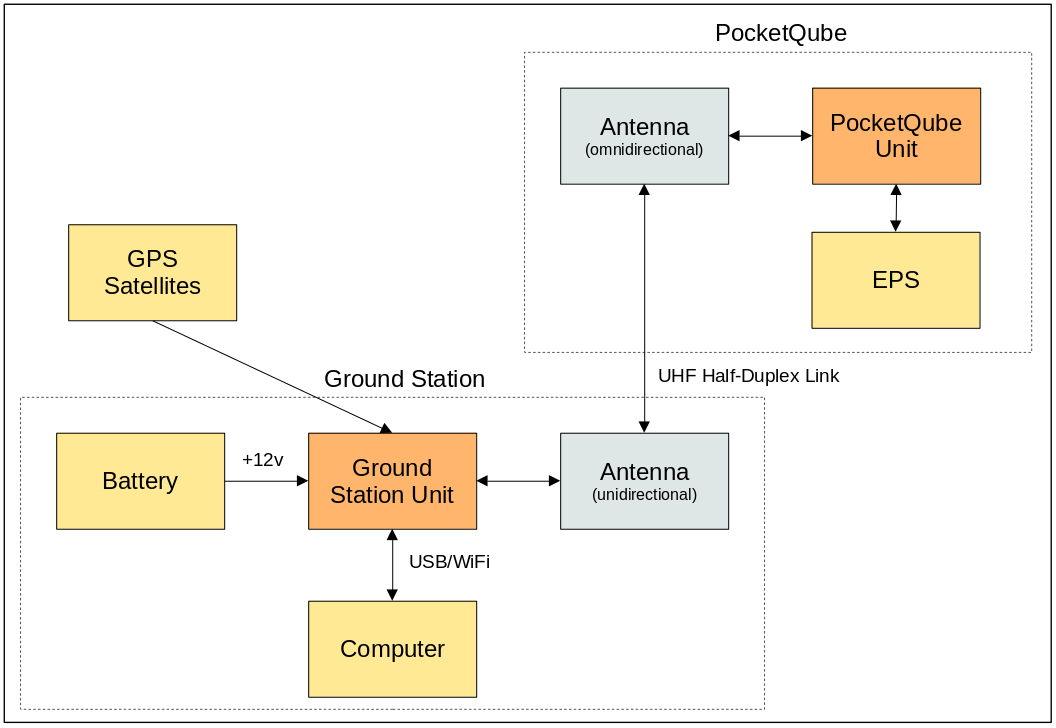
\includegraphics[width=0.8\textwidth]{complete_system.png}
    \caption{High-Level System Diagram}
    \label{fig:complete_system}
  \end{figure}

\newpage
\subsection{Methodology}
Since a large number of sub-system are required on the ground-station, either \textit{modules} or simple \textit{reference designs} will be form the basic building blocks of the system. This will simplify the design process and integration. Only if no modules or designs are found to meet the system requirements, should a more custom solution be developed. The ground station will be powered via +12V from a nearby vehicle, and the PocketQube will be powered from an on-board EPS (another PQ unit). Both sub-systems should be designed such that testing without a vehicle/EPS is also possible.

\subsection{Tracking}
It is known that open-loop path-predicted tracking is adequate for high-altitude balloons. In this sense, the ground station requires at least a GPS connection, as well as some form of inertial measurement unit (IMU) for beem steering. The path data will be uploaded to the ground station via USB or WiFi and an external device, such as a laptop, personal computer or smartphone (referred to as the system's \textit{computer} onwards). Further, this computer will be used to monitor the link and record the data. If longer-range communication is required, it will be desirable to have a second method of tracking other than path prediction. Either radio signal-strength tracking, or direct GPS tracking, may then be added.

\subsection{Custom Protocol}
Firstly, high-level decisions should be made regarding the custom communication protocol to be implemented. Half-duplex communication will be designed for, since full-duplex is unnecessary for this type of link. This is due to the nature of the link itself i.e. the command-response pattern used when receiving data from satellites.

For the given flight path, a goal of at least 9600 downlink baud rate will be designed for at the approximate 100 km range, as it is a relatively standard satellite downlink speed as mentioned. Both GFSK and LoRa techniques will be explored in the detailed design stage, since GFSK is well-estabilished and is considered suitable over such a range, but LoRa may have added noise immunity benefits.

\subsection{Proprietary Protocol}
The requirement to communicate with the existing Radiosonde should be considered. According to the iMet54's datasheet \cite{datasheet-iMet54}, it operates at a centre frequency of between 402 and 405 MHz, selected in 1 MHz increments. Ideally, for a simpler design, one antenna should be designed on the GS supporting both the custom and proprietary communication communication protocols. The feasibility of this will be investigated further in the antenna design stage.

\newpage
\subsection{Phased Design Plan}
If very long-range communication is to be supported, a highly-directive antenna will most likely be needed and, as mentioned in Section \ref{sec:antenna_theory}, these antennas are usually large in size. Although the possibility of a high-gain design in the 400 to 500 MHz band will be investigated, it is probable that this may be limited by the size and weight constraints of the existing antenna mount. Given the above considerations, it was decided for the detailed design to follow a phased approach:
\begin{itemize}
  \item \textbf{Phase 1:} The design of a single ground station antenna in the 400 to 500 MHz band, allowing for close-range testing of both the custom and proprietary protocols. Only open-loop tracking will be implemented.
  \item \textbf{Phase 2:} The addition of a physically smaller, high-gain 868 MHz band antenna for long-range custom protocol communication. Signal-strength tracking, as well as GPS on the satellite, may be added.
\end{itemize}

\noindent In this way, close-range system requirements are met in Phase 1, and longer range support can be added in Phase 2, if time allows. This phased-approach is also made possible due to the choice to use modular components, which easily allows e.g. a 433 MHz RF module to be swapped for an 868 MHz module, with minimal re-design.